\chapter{Thermal Hydraulics}
\label{ch:thermalHydraulics}

\section{Introduction}
  For reactor design purposes, designs are ultimately constrained by thermal
  properties. Additionally, neutronics properties in the form of cross sections
  and density changes are significantly affected by system temperatures.
  Therefore, to accurately simulate the neutron distribution within the reactor,
  it is necessary to also simulate temperatures within the reactor.

  In this simulation, two thermal hydraulic models are
  employed. The first is a one-dimensional fluid flow model to calculate coolant
  temperatures as the coolant flows through a channel. This model is valid for
  the assumption of no cross-flow between channels and perfect fluid mixing 
  within the flow channel. For use in simulating fast reactors with canned
  assemblies and assembly designs which encourage mixing, these assumptions are
  valid. The second model used is a radial
  pin-conduction model to calculate cladding, sodium bond, and fuel temperatures
  based on the heat conduction equation.

  Thermodynamic properties of reactor materials are required for these models.
  The sodium properties required are the most extensive with density, enthalpy, 
  thermal conductivity, dynamic viscosity, and heat capacity required. The 
  functional forms of these properties in this application are given in 
  \cite{sodiumProp}. Additionally, thermal conductivity values are required for 
  cladding and fuel material. Typical cladding for fast reactor designs is HT9
  stainless steel and a functional form of the conductivity is given in
  \cite{ht9Prop}. Fuel composition is assumed to be of the form U-Zr$x$ where
  $x$ is the weight fraction of Zr in the fuel. A typical value for x is 10\%.
  Fuel thermal conductivity is given in \cite{fuelProp}. For the expression of
  fuel thermal conductivity given, the integral of thermal conductivity 
  is unbounded as $T \rightarrow 0$ so thermal conductivity is assumed
  constant below 300 K which is below the melting point of sodium so this
  assumption is valid for reactor applications.

\section{Geometric Description}
  For the purposes of the thermal hydraulics model, geometry is described in
  \fref{fig:radial_model}. This model represents a cylindrical fuel pellet,
  surrounded by sodium bond, enclosed in steel cladding, with sodium coolant
  flowing in the axial direction. The center of the fuel pin is located at
  $r=0$ where $r$ is the radial coordinate. The fuel pellet has radius $R_F$ and
  fuel is located in $r \in [0,R_F)$. Then, bond is located in $r \in (R_F,R_B)$
  and clad is located in $r \in (R_B,R_C]$. The fuel center-line temperature is
  $T_0$ and fuel surface temperature is $T_F$. Bond surface temperature is
  $T_B$ and clad surface temperature is $T_C$. $T_{\infty}$ represents the bulk
  coolant temperature. In this model, heat is generated exclusively in the fuel
  with volumetric heat generation rate $q'''$. 

  In a cross-sectional assembly view, dimensions are presented in
  \fref{fig:pin_model} and \fref{fig:hex_can}. In \fref{fig:hex_can}, $Th_{Box}$
  is the thickness of the assembly box, F2F is the flat-to-flat measurement of
  the outside of the hexagonal can, and Pitch is the distance between the
  center of two pins. In future notation, the quantity ``Pitch'' is also noted
  $S$. Using the geometry described in these figures, the material
  cross-sectional areas are calculated according to the given formulae where
  $N_{pin}$ is the number of pins in the assembly.
  \begin{align}
    A_{total} &= \frac{\sqrt{3}}{2} F2F^2 \\
    A_{can} &= A_{total} - 
      \frac{\sqrt{3}}{2} \left(  F2F - 2 \, Th_{Box} \right) \\
    A_{wrap} &= N_{pin} \frac{\pi}{4} D_{wrap}^2 \\
    A_{clad} &= N_{pin} \pi (R_C^2 - R_B^2) \\
    A_{bond} &= N_{pin} \pi (R_B^2 - R_F^2) \\
    A_{fuel} &= N_{pin} \pi R_F^2 \\
    A_{cool} &= A_{total} - A_{can} - A_{wrap} - A_{clad} - A_{bond} - A_{fuel}
  \end{align}
  Calculating the areas as above allows for calculation of cross-sectional area
  fractions. Assuming constant dimensions within an element in the axial
  direction, these area fractions are equivalent to volume fractions and are
  useful for neutron cross section calculations. Additionally, these formulae
  allow for thermal expansion calculations as the liquid sodium in the bond and
  the coolant are allowed to vary to allow for the expansion of other materials.

  \begin{figure}
    \centering
    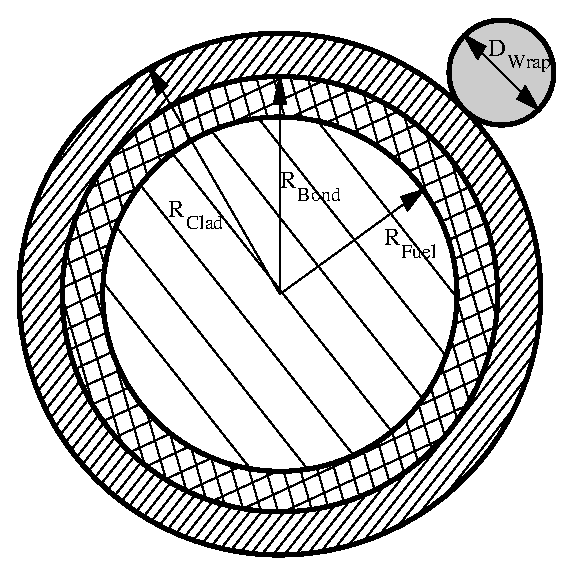
\includegraphics[width=0.5\textwidth]{pin_model}
    \caption{Dimensions of Thermal Hydraulic Pin Model.}
    \label{fig:pin_model}
  \end{figure}

  \begin{figure}
    \centering
    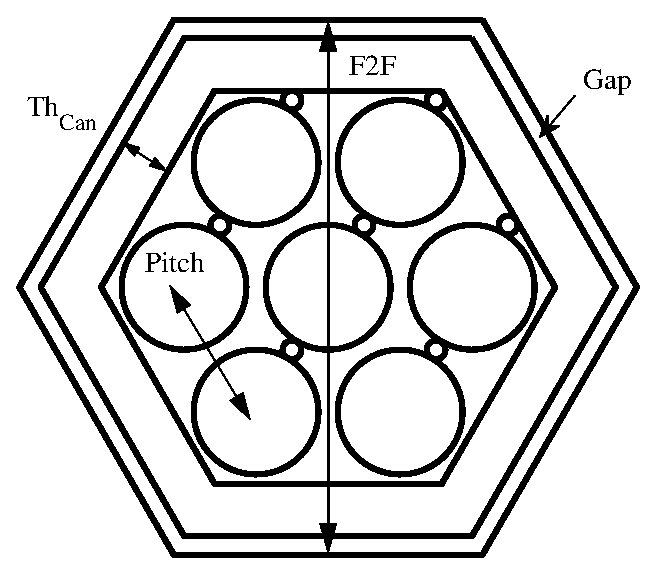
\includegraphics[width=0.5\textwidth]{hex_can}
    \caption{Dimensions of Hexagonal Can.}
    \label{fig:hex_can}
  \end{figure}
  
  \begin{figure}
    \centering
    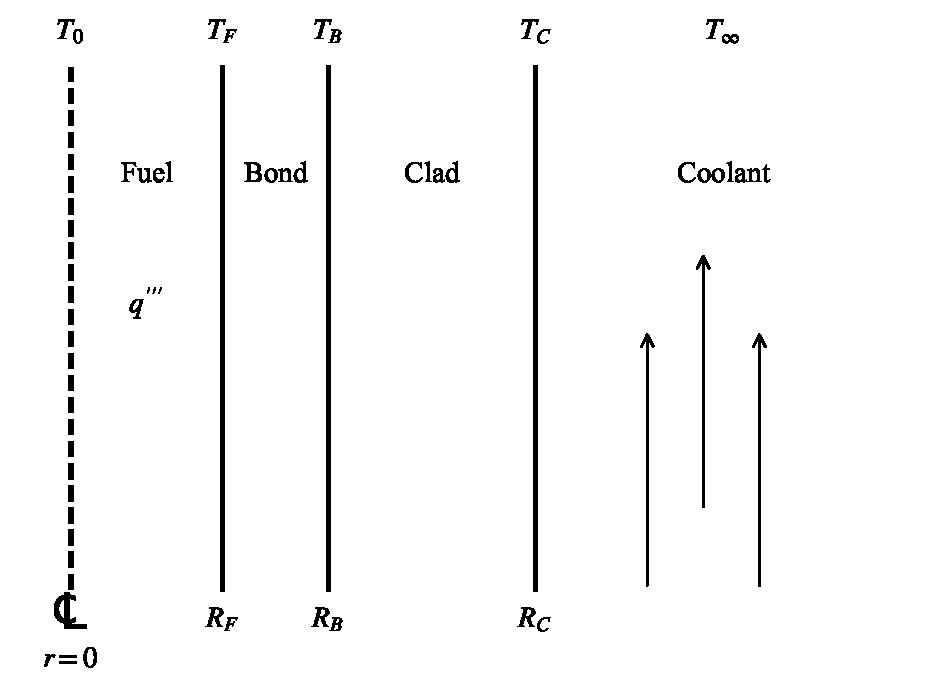
\includegraphics[width=0.5\textwidth]{radial_model}
    \caption{Geometry Description for Thermal Hydraulics Model.}
    \label{fig:radial_model}
  \end{figure}

  Used in association with an unstructured mesh, the thermal hydraulic model
  requires mapping mesh elements to flow channels. In the user input to the
  program, the user must specify to which one-dimensional flow channel belongs.
  Adopting the nomenclature from fast reactors, each flow channel represents a
  hexagonal-assembly or a ``hex''. In the following discussion, a hex index is
  subscripted $h$ for $h = 1,2,\ldots,N_h$ where $N_h$ is the number of
  hexagonal assemblies in a reactor. Though the term ``hex'' is used, there is
  no assumption made in any of the calculations that the assembly is indeed
  hexagonal. Square one-dimensional assemblies would be simulated similarly.

  The concept of ``chunks'' is also introduced to aid in the discretization of
  the thermal hydraulic model. A chunk is the set of all elements in a channel
  with a unique axial elevation. For example, in a fast reactor hexagonal
  assembly, the assembly has a unique $h$ index and contains a number of chunks
  equal to the number of axial elevations in the simulation. Additionally, each 
  chunk is required to have unique material composition. The concept of chunks
  is shown in \fref{fig:chunk_description}.  Chunks are indexed
  $c = 1,2,\ldots,N_c$ where $N_c$ is the total number of chunks. For $N_z$
  axial elevations, $N_c = N_h \, N_z$. The indexing
  of chunks is chosen such that $c+N_h$ is the chunk one axial elevation above
  chunk $c$. 

  \begin{figure}
    \centering
    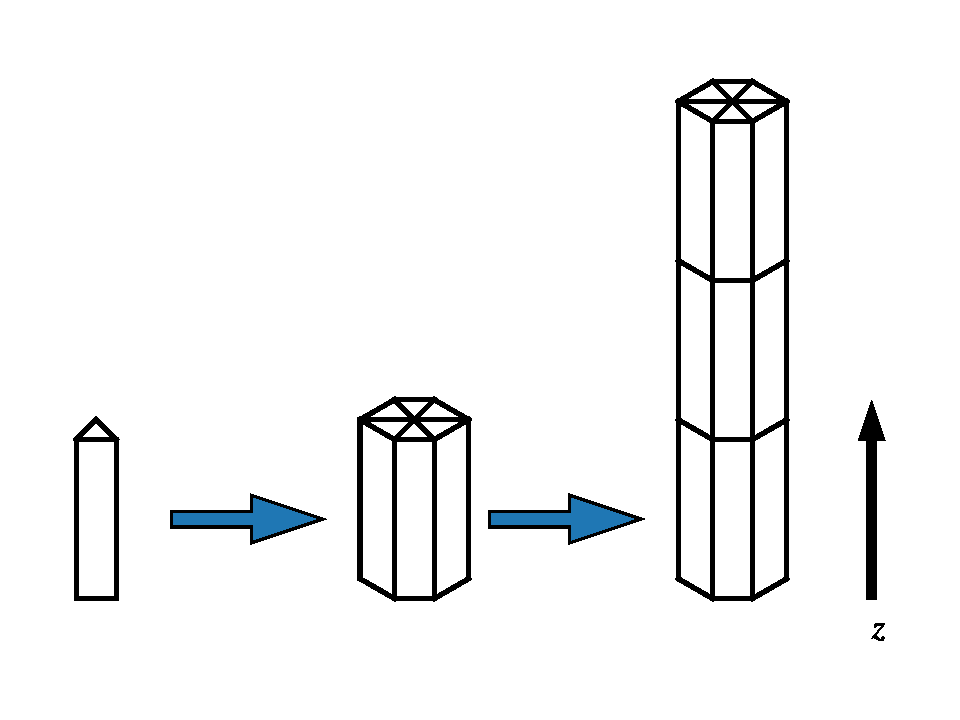
\includegraphics[width=0.7\textwidth]{chunk_description}
    \caption{Progression of Element (left), to Chunk (center), to Hex (right).}
    \label{fig:chunk_description}
  \end{figure}

\section{Power Calculation}
  Recall the multigroup neutron diffusion equation solved via the power
  iteration method returns the largest eigenvalue $\keff$ and unique positive
  eigenvector $\phi_g$ (see \sref{sec:power_iterations}). The flux calculated
  according to this method can be normalized to an arbitrary constant. For a
  specified total reactor power, $Q_{Rx}$ the normalization constant can be 
  calculated. For un-normalized neutron flux $\widetilde{\phi_{g,e}}$ with group
  $g$ in element $e$, the normalization constant is written as
  \begin{equation}
    \label{eq:normalization_c}
    c = \frac{Q_{Rx}}{\sum_{g}^{G} \sum_{e}^{N_E} \kappa \Sigma_{f,g,e} \,
      \widetilde{\phi_{g,e}}}
  \end{equation}
  where $c$ is the normalization constant. $\kappa$ represents the reclaimable
  (non-neutrino) energy produced per fission such that the quantity $\kappa
  \Sigma_f \phi$ represents the heat generation rate. Then the true reactor
  neutron flux is given as
  \begin{equation}
    \label{eq:normalization_phi}
    \phi_{g,e} = c \, \widetilde{\phi_{g,e}}
  \end{equation}
  and the power distribution is 
  \begin{equation}
    \label{eq:normalization_q}
    q_{e} = \sum_g^G \kappa \Sigma_{f,e,g} \phi_{g,e}.
  \end{equation}
  For an elemental power $q_e$, then the volumetric heat generation rate within
  the fuel is 
  \begin{equation}
    \label{eq:elementqppp_fuel}
    q'''_{e} = \frac{q_e}{V_{fuel,e}}
  \end{equation}
  where $V_{fuel,e}$ is the volume of fuel in element $e$. This will be
  necessary for the radial conduction model.

  For the one-dimensional heat convection model in the axial direction,
  heat generation quantities are needed for chunks instead of elements.
  The quantities required are then the total heat generated in a chunk $q_c$ and
  the average volumetric heat generation rate in the fuel for elements within
  the chunk $q'''_c$. These relationships are given in \eref{eq:chunkpwr} and
  \eref{eq:chunkqppp_fuel} respectively. The notation $e \in c$ implies the
  summation over all elements $e$ within chunk $c$.
  \begin{align}
    \label{eq:chunkpwr}
    q_c = \sum_{e \in c} q_e \\
    \label{eq:chunkqppp_fuel}
    q'''_c = \frac{\sum_{e \in c} q'''_e V_{fuel,e}}{\sum_{e \in c} V_{fuel,e}}
  \end{align}

\section{Axial Convection Model}
  First, the channel mass flow $\mdot_h$ must be calculated for a user specified
  total reactor mass flow rate $\mdot_{Rx}$.  Mass flow is partitioned into each
  channel assuming constant mass flux at the reactor inlet according to 
  \begin{equation}
    \label{eq:mass_flow_split}
    \mdot_h = \mdot_{Rx} \frac{A_{cool,h}}{A_{cool,Rx}}
  \end{equation}
  where $A_{cool,h}$ is the coolant flow area for channel $h$ and $A_{cool,Rx}$
  is the coolant flow area for the reactor.  That is, the mass 
  flow per unit area is assumed constant at the reactor inlet and the mass flow 
  in a channel is the product of the mass flux and the channel flow area. 
  
  The coolant enthalpy for an axial location $z$ within the channel is expressed
  by a simple heat balance equation as
  \begin{equation}
    \label{eq:continuous_heat_balance}
    h_h(x) = h_{in} + \frac{1}{\mdot_h} \int_0^z q'_h(z') \; dz'
  \end{equation}
  where $h$ is the specific enthalpy, $h_{in}$ is the inlet enthalpy, $\mdot_h$
  is the mass flow rate within the channel, and $q'_h(x)$ is the linear heat 
  generation rate for channel $h$ at elevation $z$. $h_{in}$ is related to a
  user specified 
  $T_{inlet}$ by a state relationship for the coolant $h_{in} = h(T_{inlet})$.
  The integral in \eref{eq:continuous_heat_balance} can be discretized along the
  channel and converted to a summation.
  \begin{equation}
    \label{eq:heat_balance}
    h_c = h_{in} + \frac{1}{\mdot_h} \sum_{i}^{N_z} q'_{i,h} \Delta z_{i,h}
  \end{equation}
  where $q'_{i,h}$ is the linear heat generation rate in the chunk located at 
  axial level $i$ in 
  channel $h$ and $\Delta z_{i,h} = z_{i+1,h} - z_{i,h}$. (Note: by indexing
  properly, $c = h + (i-1) \, N_h$.) Recognizing the 
  quantity $q'_{i,h} \Delta z_{i,h}$ is the total heat generated in channel $h$ 
  at axial level $h$, then \eref{eq:heat_balance} can be rewritten.
  \begin{equation}
    h_c = h_{in} + \frac{1}{\mdot_h} \sum_i^{N_z} q_{i,h}
  \end{equation}
  The final result of this model is $h_c$, the bulk coolant enthalpy in each
  chunk $c$. Given, $h_c$, bulk coolant temperature $T_{\infty,c} = T(h_c)$ can
  be calculated using a state relationship. This will be an input into the 
  Radial Conduction Model, \sref{sec:radial_conduction_model}, to later 
  calculate the average material temperatures.
  
\section{Radial Conduction Model}
  \label{sec:radial_conduction_model}
  \subsection{Surface Temperature and Center-Line Temperatures}
    \subsubsection{Clad Surface Temperature}
    \subsubsection{Bond Surface Temperature}
    \subsubsection{Fuel Surface Temperature}
    \subsubsection{Fuel Center-Line Temperature}
  \subsection{Average Temperatures}
\section{Cross Section Treatment}
  \subsection{Cross Section Library Generation}
  \subsection{Temperature Dependent Cross Section Calculation}

% todo this will probably be a separate chapter and include thermal expansion
%\section{Results}
%  \subsection{Single Pin Model}
%  \subsection{Reactor Simulation}
